\documentclass{beamer}
\usepackage{physics}
\usepackage{hyperref}

%Information to be included in the title page:
\title{Numerical bootstrap}
\author{Jinyuan Wu}
\institute{Department of Physics, Fudan University}
\date{2021}

\usetheme{Madrid}

\newcommand{\concept}[1]{\textbf{#1}}

\begin{document}

\frame{\titlepage}

\begin{frame}
\frametitle{Introduction}

\textbf{What's bootstrap}

\begin{itemize}
    \item A quantum theory = expectations of all Hermitian operators; 
    Hamiltonian/Lagrangian $\Leftrightarrow$ ``probability distribution''
    \item Constraint on the system $\Rightarrow$ relation between different $\expval{O}$'s (``\concept{data}'');
    independent $\expval{O}$'s $\Leftrightarrow$ parameters in the model
    \item Inequality constraint (e.g. positivity of $\expval{O^\dagger O}$) $\Rightarrow$ quantum allowed 
    range of $\expval{O}$'s
    \item Solving a class of problems without mentioning explicitly the wave function/path integral: 
    hence the name \emph{bootstrap}
\end{itemize}

\vspace{1em}

\textbf{Why we need it}

\begin{itemize}
    \item Because it doesn't fail with strong non-perturbative effects. \footnote{See \href{https://arxiv.org/abs/2108.11416}{arXiv 2108.11416}.}
\end{itemize}

\end{frame}

\begin{frame}
\frametitle{Example: conformal bootstrap}

\begin{itemize}
    \item The most famous example: \concept{conformal bootstrap}
    \item Constraints: (spinless) two-point function 
    \begin{equation}
        \expval*{\mathcal{O}(x) \mathcal{O}(y)} = \frac{1}{\abs*{x - y}^{2 \Delta_\mathcal{O}}},
    \end{equation}
    three-point function 
    \begin{equation}
        \begin{aligned}
            &\quad \langle\mathcal{A}(x) \mathcal{B}(y) \mathcal{C}(z)\rangle \\
            &= \frac{f_{\mathcal{A B C}}}{|x-y|^{\Delta \mathcal{A}+\Delta_{\mathcal{B}}-\Delta_{\mathcal{C}}}|y-z|^{\Delta_{\mathcal{B}}+\Delta_{\mathcal{C}}-\Delta \mathcal{A}}|z-x|^{\Delta_{\mathcal{C}}+\Delta_{\mathcal{A}}-\Delta_{\mathcal{B}}}}
        \end{aligned}
    \end{equation}
    Higher order correlation functions: OPEs. 
    \item Independent parameters: $\{\Delta_{\mathcal{O}}, l_{\mathcal{O}}, f_{\mathcal{A} \mathcal{B} \mathcal{C}}\}$
    \item Inequality constraints (self-consistent conditions): determining the range of parameters
\end{itemize}

\end{frame}

\begin{frame}
\frametitle{Example: conformal bootstrap}

\begin{itemize}
    \item Example of conformal bootstrap: verify whether the critical point of 3D Ising model 
    is a CFT \footnote{\href{https://arxiv.org/abs/1203.6064}{1203.6064} }
    \item Physical picture tells us there are two fields: energy density $\epsilon$, spin field $\sigma$
    \item Below is Fig.~3 in the paper: comparing critical exponents from Monte Carlo simulation of 3D Ising, and the allowed range from conformal bootstrap
\end{itemize}

\begin{center}
    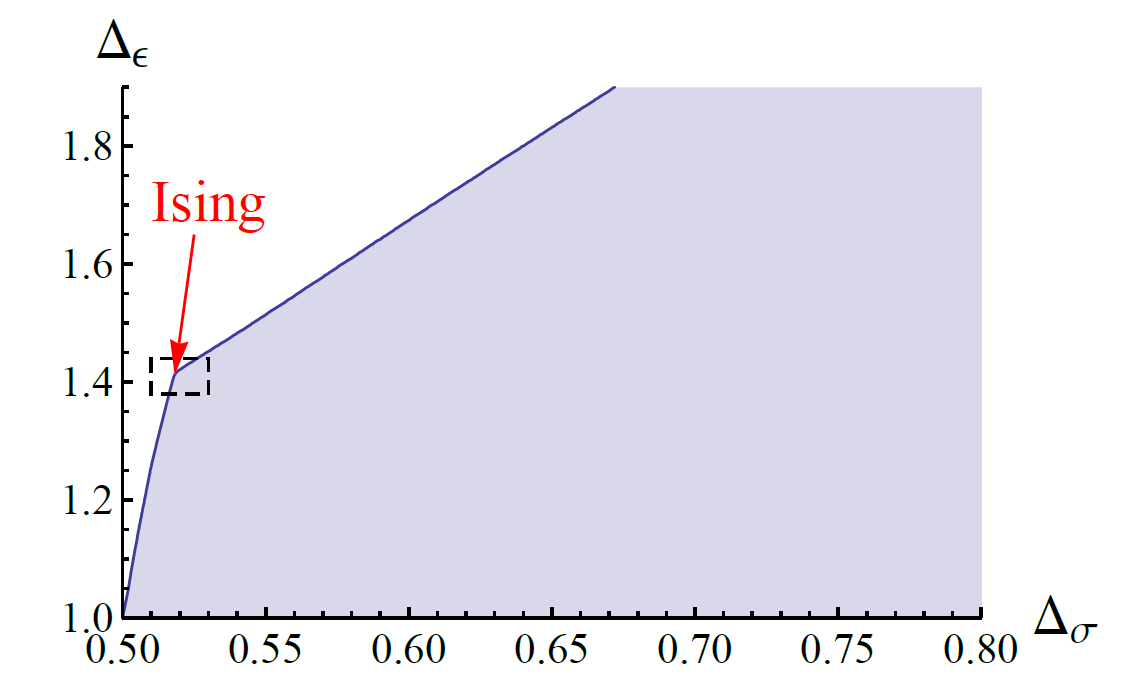
\includegraphics[width=0.5\textwidth]{3d-ising-cft-bootstrap-range.PNG}
\end{center}

\end{frame}

\end{document}